\documentclass[11pt]{article}
\usepackage{tipa}
\usepackage{graphicx}
\usepackage[hmargin=2cm,vmargin=2cm]{geometry}
\geometry{a4paper}

\usepackage{fancyhdr} % This should be set AFTER setting up the page geometry
\pagestyle{fancy} % options: empty , plain , fancy
\renewcommand{\headrulewidth}{0pt} % customise the layout...
\lhead{}\chead{}\rhead{}
\lfoot{}\cfoot{\thepage}\rfoot{}

\title{title here}
\date{}

\begin{document}

\begin{center}
	\textbf{Acoustics of coronal stops in Spanish-English bilingual speech}
\end{center}

Spanish and English possess a contrast between fortis (/p t k/) and lenis stops (/b d g/); however, the phonetic implementation of this contrast differs for the two languages. The primary acoustic-phonetic correlate of the fortis-lenis contrast is Voice Onset Time (Lisker and Abramson, 1964). The differences between Spanish and English with respect to how they use VOT in stops have been examined in numerous occasions. Importantly, in addition to VOT, Spanish and English coronal stops differ in their place of articulation: Spanish /d/ and /t/ are commonly described as dental and English /d/ and /t/ are described as alveolar. How is this reflected on the acoustic signal? Previous research has shown that some spectral moment measurements of the stop burst are able to capture the aforementioned place difference. Sundara (2005), for instance, found that Canadian French, whose /d/ and /t/ are dental, and English coronal stops differed in relative burst intensity, center of gravity, standard deviation, and kurtosis. More recently, Casillas et al. (2015) found that standard deviation and center of gravity could accurately predict phoneme identity for Spanish and English short-lag stops (English /d/ \emph{vs.} Spanish /t/). This opened the door to new questions pertaining to bilingual populations: How do Spanish-English bilinguals manage the differences between these two languages with respect to how /d/ and /t/ are produced? Is the place difference exploited at all in bilingual speech? The present study analyzes the acoustics of coronal stops in order to examine the effects of bilingualism on these consonants.

The present study compares the speech of two groups of Spanish-English bilinguals (English- \emph{vs.} Spanish-dominant), a group of Spanish monolinguals and a group of English monolinguals. Using professional equipment, eight native English speakers were recorded in Arizona and eight Spanish speakers were recorded in Spain. Additionally, sixteen Spanish-English sequential bilinguals were recorded in Arizona. All of the speakers were females. The bilinguals, fluent \emph{heritage} Spanish speakers born and raised in Arizona, were subdivided into two groups based on language dominance according to a comprehensive survey that inquired about language experience, use, proficiency and attitudes. Speakers produced target words with /d/ and /t/ in utterance-initial position. Word-initial syllables were orthogonally controlled for lexical stress (stressed, prestressed). Production data were collected with the delayed shadowing technique. Six male ``talkers'' (3 Spanish, 3 English) originally recorded the materials and these stimuli were then played in random order to the speakers, who were asked to ``listen and repeat the sentences.'' We obtained a total of 3,456 tokens. The data were submitted to acoustic scrutiny; in addition to VOT, we analyzed the statistics of the spectrum of the burst from a 30 ms Gaussian window left-aligned with the burst. After Casillas et al. (2015), we focused on center of gravity and standard deviation.

The data, which were analyzed using linear mixed-effects models and are ready to be reported, indicated the following: coronal production varied as a function of language as well as, in bilinguals, language dominance. For English coronals, we found that VOT of short-lag stops decreased as dominance in Spanish increased. Specifically, when compared with the monolingual control group, the English-dominant bilinguals produced more tokens of /d/ with lead VOT, and the Spanish dominant bilinguals produced even more. There were no group differences based on standard deviation and center of gravity. For Spanish coronals, there were group differences for center of gravity, suggesting that the place for Spanish /d/ and /t/ became more variable with increased dominance in English. Finally, an analysis of the bilingual groups' productions of short-lag stops (English /d/ \emph{vs.} Spanish /t/) showed that both groups distinguished between Spanish and English using VOT and various spectral moments, regardless of language dominance. The VOT difference is attributed to the bilingual groups' tendency to occasionally produce English stops with lead VOT, and the spectral differences are attributed to the place differences between Spanish and English.

The present study examined the acoustics of Spanish and English /d/ and /t/. In particular, it set out to examine whether bilingualism and, then, language dominance affect the production of the two aforementioned languages. The results suggest this to be the case. Importantly, the analysis of short-lag stops suggests that early bilinguals maintain separate categories for coronal stops in each of their languages thereby exploiting phonetic features that go beyond the ones previously described.


\pagebreak

\begin{figure}[!h]
	\centering
	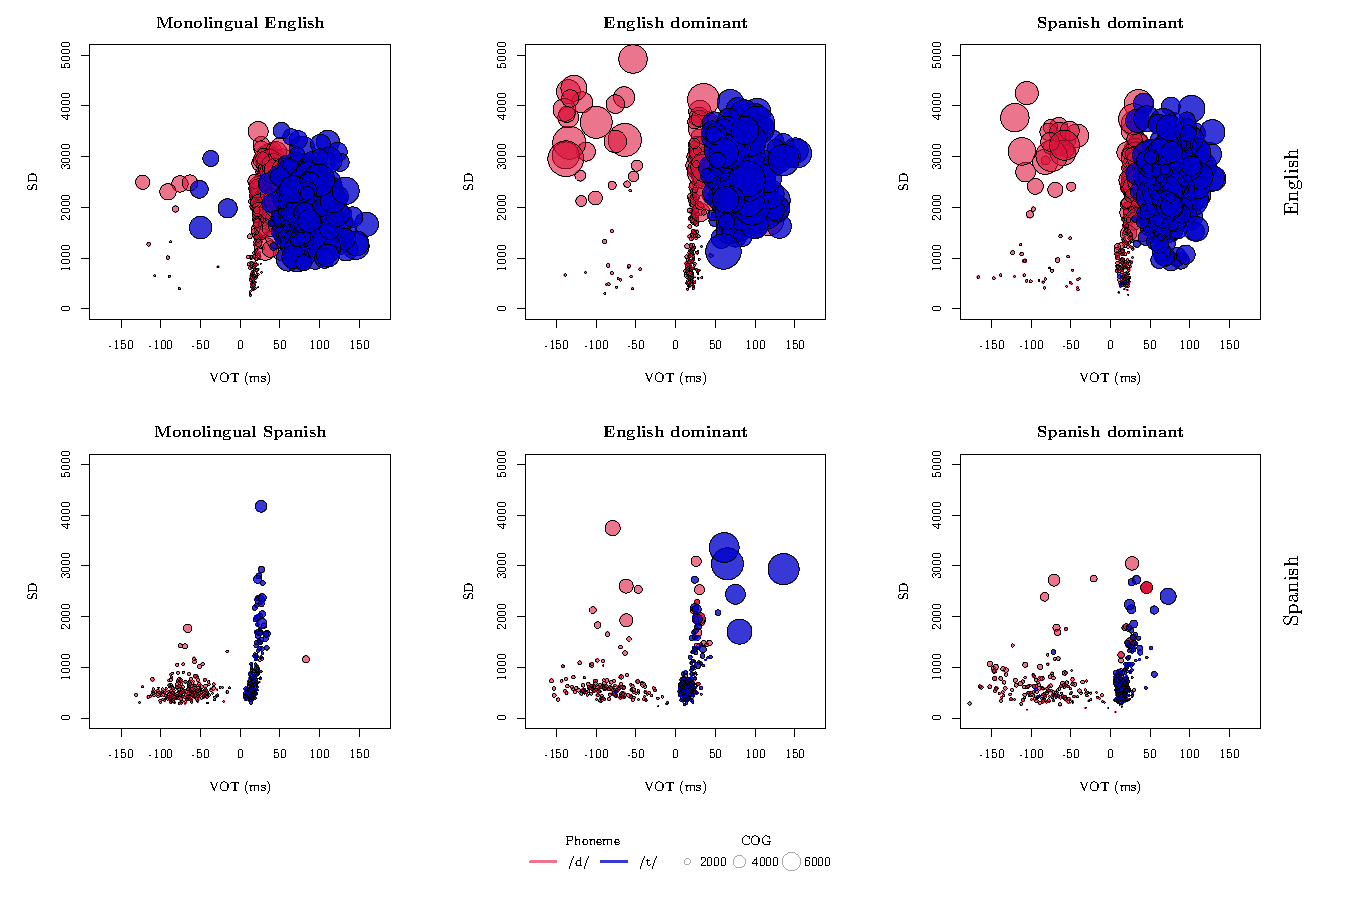
\includegraphics[width=\textwidth]{figures/all.pdf}
	\caption{VOT, SD, and COG as a function of phoneme (/d/, /t/), language (Spanish, English), and linguistic experience (monolingual, Spanish dominant, English dominant). The y-axis plots SD, the x-axis plots VOT, and COG is expressed via point size.}
	\label{fig:1}
\end{figure}

\begin{figure}[!h]
	\centering
	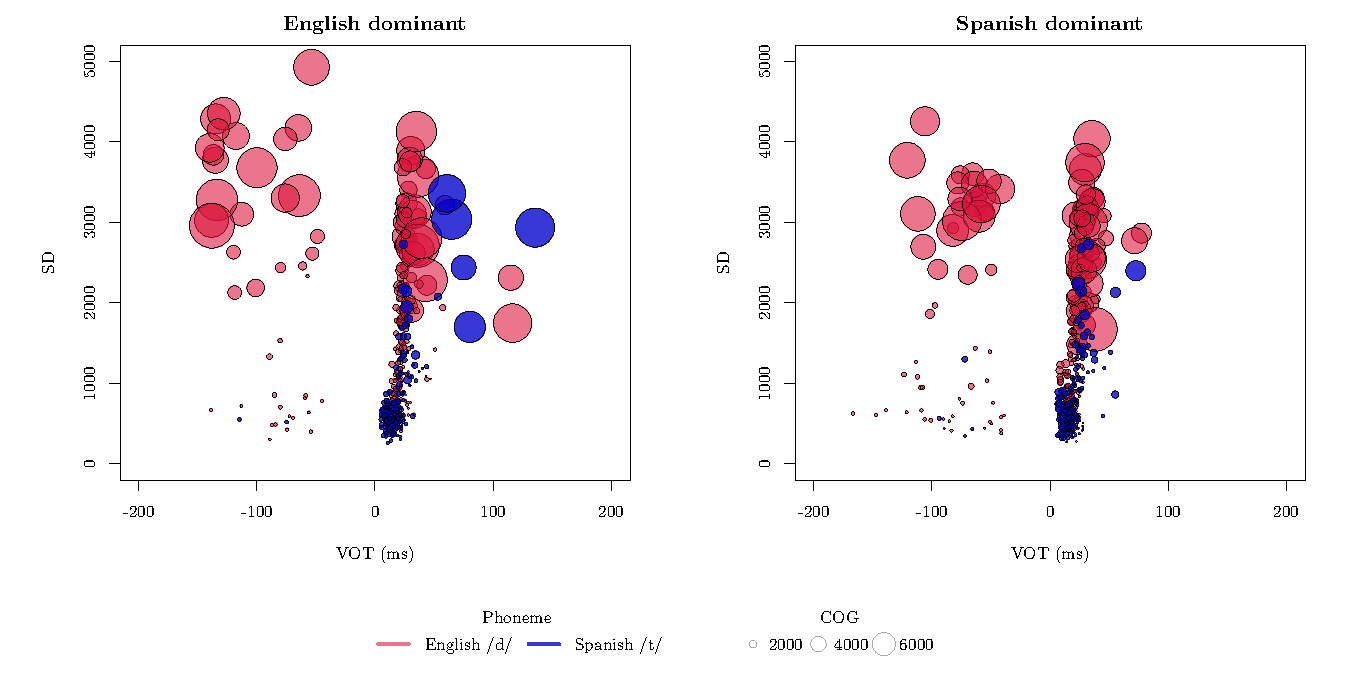
\includegraphics[width=.65\textwidth]{figures/dt_compare.pdf}
	\caption{VOT, SD, and COG of short-lag stops (Spanish /t/, English /d/) as a function of linguistic experience (Spanish dominant, English dominant). The y-axis plots SD, the x-axis plots VOT, and COG is expressed via point size.}
	\label{fig:2}
\end{figure}



\end{document}



